\begin{tabular}{cc}
\scalebox{0.5}{
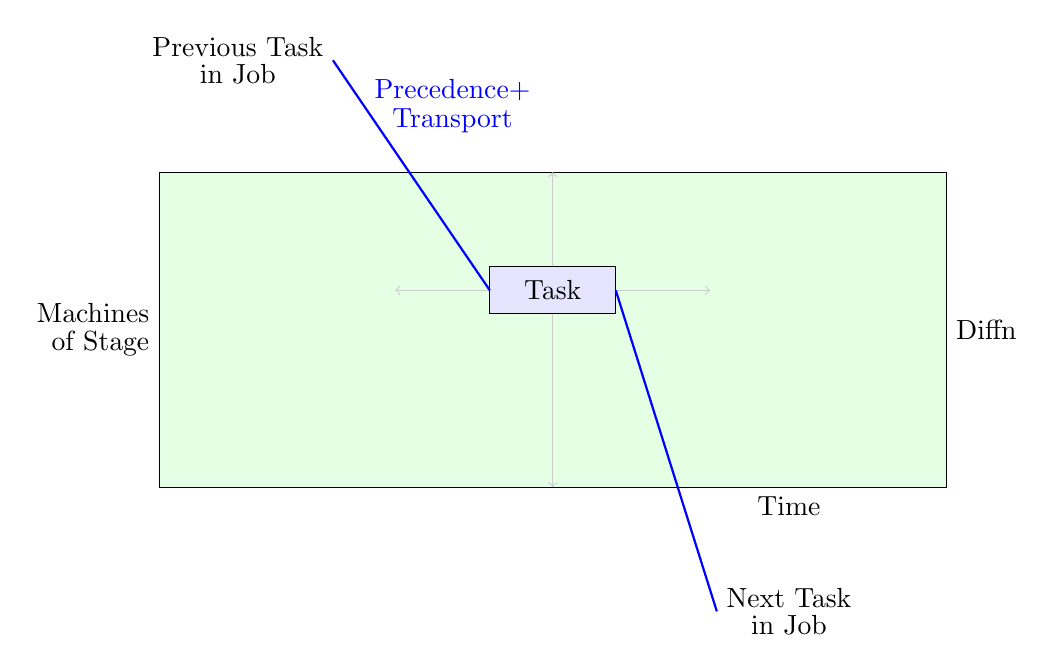
\begin{tikzpicture}
  \draw[draw=black,fill=green!10] (0,0) rectangle (10,4);
  \node[right] () at (10,2.0) {Diffn};
  \draw[black!20,<->] (3,2.5) -- (7,2.5);
  \draw[black!20,<->] (5,0) -- (5,4);
  \draw[fill=blue!10] (4.2,2.2) rectangle node {Task} (5.8,2.8);
  \node[below] (time) at (8,0) {Time};
  \node[left] (machine) at (0,2) {\shortstack[r]{Machines\\of Stage}};
  \node[above] (prev) at (1,5) {\shortstack{Previous Task\\in Job}};
  \node[above] (next) at (8,-2) {\shortstack{Next Task\\in Job}};
  \draw[thick,blue] (prev.east) -- node[pos=0.2,right] {\shortstack{Precedence+\\Transport}} (4.2,2.5);
  \draw[thick,blue] (next.west) -- (5.8,2.5);
\end{tikzpicture}
}
&
\scalebox{0.5}{
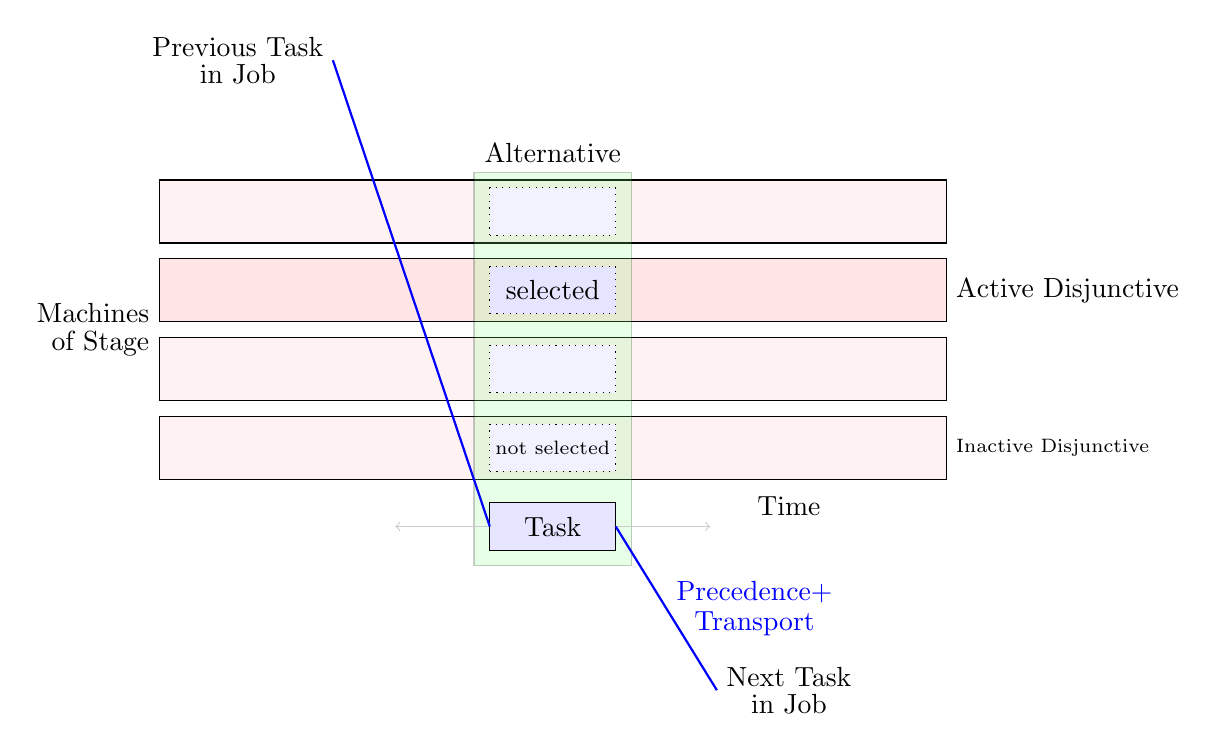
\begin{tikzpicture}
  \draw[draw=black,fill=red!5] (0,0.1) rectangle (10,0.9);
  \draw[draw=black,fill=red!5] (0,1.1) rectangle (10,1.9);
  \draw[draw=black,fill=red!10] (0,2.1) rectangle (10,2.9);
  \draw[draw=black,fill=red!5] (0,3.1) rectangle (10,3.9);
  \node[right] () at (10,2.5) {Active Disjunctive};
  \node[right] () at (10,0.5) {\scriptsize Inactive Disjunctive};
  \draw[fill=green!50,opacity=0.2] (4,-1) rectangle (6,4);
  \node[above] () at (5,4) {Alternative};
  \draw[dotted,fill=blue!5] (4.2,0.2) rectangle node {\scriptsize not selected} (5.8,0.8);
  \draw[dotted,fill=blue!5] (4.2,1.2) rectangle (5.8,1.8);
  \draw[dotted,fill=blue!10] (4.2,2.2) rectangle node {selected} (5.8,2.8);
  \draw[dotted,fill=blue!5] (4.2,3.2) rectangle (5.8,3.8);
  \draw[black!20,<->] (3,-0.5) -- (7,-0.5);
  \draw[fill=blue!10] (4.2,-0.2) rectangle node {Task} (5.8,-0.8);
  \node[below] (time) at (8,0) {Time};
  \node[left] (machine) at (0,2) {\shortstack[r]{Machines\\of Stage}};
  \node[above] (prev) at (1,5) {\shortstack{Previous Task\\in Job}};
  \node[above] (next) at (8,-3) {\shortstack{Next Task\\in Job}};
  \draw[thick,blue] (prev.east) -- (4.2,-0.5);
  \draw[thick,blue] (next.west) -- node[right] {\shortstack{Precedence+\\Transport}} (5.8,-0.5);
\end{tikzpicture}
}
\end{tabular}
